\chapter*{Proposition 11}
\label{prop:11}


\begin{figure*}[ht]
    \begin{center}
    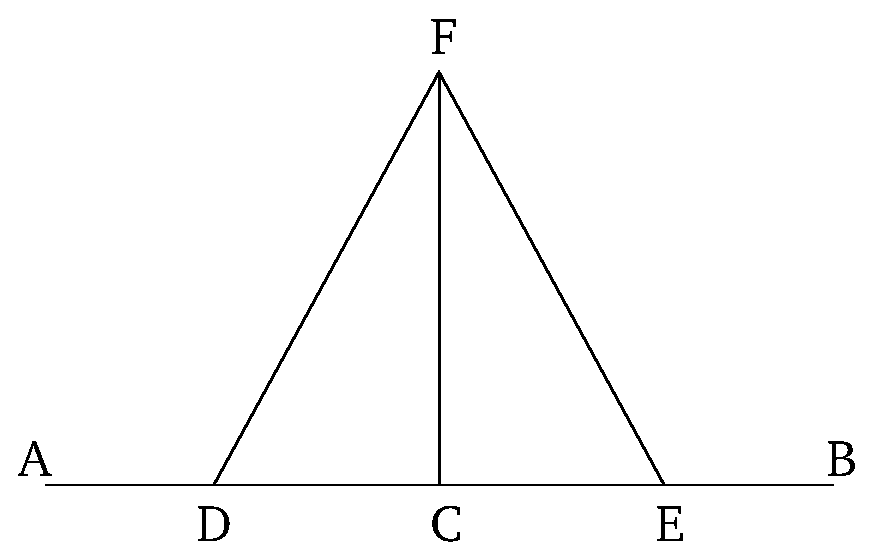
\includegraphics[width=0.5\linewidth]{figures/fig11e.eps}
    \label{fig:prop_11}
    \end{center}
\end{figure*}

To draw a straight-line at right-angles to a given straight-line from a given point on it.

Let $AB$ be the given straight-line, and $C$ the given point on it. So it is required
to draw a straight-line from the point $C$ at right-angles to the straight-line $AB$.

Let the point $D$ be have been taken at random on $AC$, and let $CE$ be made equal to $CD$ [Prop.~1.3], and let the equilateral triangle $FDE$
have been constructed on $DE$ [Prop.~1.1], and let $FC$ have been
joined. I say that the straight-line $FC$ has been drawn at right-angles
to the given straight-line $AB$ from the given point $C$ on it.

For since $DC$ is equal to $CE$, and $CF$ is common, the two (straight-lines) $DC$, $CF$
are equal to the two (straight-lines), $EC$, $CF$, respectively.  And the base $DF$
is equal to the base $FE$. Thus, the angle $DCF$ is equal to the
angle $ECF$ [Prop.~1.8], and they are adjacent. But when a straight-line stood on 
a(nother) straight-line makes the adjacent angles equal to one another, each of the
equal angles is a right-angle [Def.~\ref{def:10}]. Thus, each of the (angles)
$DCF$ and $FCE$ is a right-angle.

Thus, the straight-line $CF$ has been drawn at right-angles to the
given straight-line $AB$ from the given point $C$ on it. (Which is) the very thing
it was required to do.


\section*{Commentary}

\begin{proposition}\label{proposition_11}\lean{Elements.Book1.proposition_11}\leanok
    $A$, $B$ are two distinct points on a line $AB$. $C$ is a point between them. Then, there must exist a point $F$ not on $AB$, s.t., $\angle~ACF$ is a right angle.
\end{proposition}
\begin{proof}
    \uses{proposition_1,proposition_3,proposition_8}\leanok
    See the original proof by Euclid.
\end{proof}

Euclid did not explicitly state that $F$ can be constructed on any side of $AB$, which is useful for later proofs.

\begin{proposition}\label{proposition_11'}\lean{Elements.Book1.proposition_11'}\leanok
    $A$, $B$ are two distinct points on a line $AB$. $C$ is a point between them, and $X$ is a point not on $AB$. Then, there must exist a point $F$ on the same side of $AB$ with $X$, s.t., $\angle~ACF$ is a right angle.
\end{proposition}
\begin{proof}
    \uses{proposition_1',proposition_3,proposition_8}\leanok
    Similar to the original proof by Euclid.
\end{proof}

Euclid's proof seems to assume $A$ and $B$ to be infinite points (so any point $C$ on the line $AB$ is between $A$ and $B$). However, infinite points are not supported in E. We need the following proposition to get around this issue.

\begin{proposition}\label{proposition_11''}\lean{Elements.Book1.proposition_11''}\leanok
    For two distinct points $A$ and $B$ on a line $AB$, there must exist a point $F$ not on $AB$, s.t., $\angle~FAB$ is a right angle.
\end{proposition}
\begin{proof}
    \uses{proposition_11}\leanok
    Let $C$ be a point on $AB$, s.t., $A$ is between $B$ and $C$. Apply Prop.~\ref{proposition_11}.
\end{proof}

Similarly, $F$ can be constructed on either side.


\begin{proposition}\label{proposition_11'''}\lean{Elements.Book1.proposition_11'''}\leanok
    $A$, $B$ are two distinct points on a line $AB$. $X$ is a point not on $AB$. Then, there must exist a point $F$ on a different side of $AB$ from $X$, s.t., $\angle~FAB$ is a right angle.
\end{proposition}
\begin{proof}
    \uses{proposition_11'}\leanok
    Let $C$ be a point on $AB$, s.t., $A$ is between $B$ and $C$. Let $Y$ be any point on the different side of $AB$ from $X$. Apply Prop.~\ref{proposition_11'}.
\end{proof}
